%========================================================= §2 IMPLEMENTATION
\section{Implementation: From-Scratch Packet Layer \& Architecture}

\subsection{Architecture and Software Module Map}
The toolkit is organized under \texttt{Imp/} as four modular, interacting packages: a low-level
shared packet layer, the offensive reconnaissance and exploitation engine, intentionally
vulnerable multi-platform lab services, and a host-based active defense countermeasure. The
delivered system layout is detailed in Table~\ref{tab:module_map}.

\begin{table}[htbp]
\centering
\small
\renewcommand{\arraystretch}{1.22}
\caption{Delivered Source Code Inventory and Component Responsibilities}
\label{tab:module_map}
\begin{tabularx}{\textwidth}{@{}L{4.4cm} X@{}}
\toprule
\hdrrow \thh{Module Path} & \thh{Engineering Role and Capabilities}\\
\midrule
\multicolumn{2}{@{}l}{\textit{\color{accent}\textbf{common/ — From-Scratch Binary Framing \& I/O Layer}}}\\
\texttt{packet.py} & Manual byte-by-byte serialization and parsing for Ethernet II, IPv4, TCP, ICMP, and UDP frames; RFC~1071 16-bit one's complement checksum engine.\\
\texttt{npcap.py} & Low-level \texttt{ctypes} bindings to Npcap and \texttt{libpcap}; packet injection, promiscuous capture, Windows IP Helper ARP resolution (\texttt{SendARP}), and adapter discovery.\\
\addlinespace
\multicolumn{2}{@{}l}{\textit{\color{accent}\textbf{attacker/ — Reconnaissance Orchestrator \& Heuristics}}}\\
\texttt{main.py} & Central attack pipeline executing Phases 1--5; CLI options for rate limiting, adapter binding, and exploit skipping.\\
\texttt{scanner.py} & Phase~1 raw Layer-2 TCP SYN half-open scanner; active diagnostic probe dispatch (ECN-SYN, SYN+FIN rule-breaker, ICMP, and UDP closed-port probes).\\
\texttt{fingerprint.py} & Phase~3 weighted probabilistic OS classification engine combining seven independent network stack heuristics.\\
\texttt{banner.py} & Phase~2 service banner grabber with protocol-aware probes (passive FTP greeting capture vs.\ active HTTP \texttt{HEAD} negotiation).\\
\addlinespace
\multicolumn{2}{@{}l}{\textit{\color{accent}\textbf{attacker/exploits/ — Dynamic, OS-Aware Exploit Battery}}}\\
\texttt{os\_payloads.py} & Phase~4 target adapter mapping OS-fingerprint tiers to targeted payloads (Windows \texttt{win.ini}/\texttt{whoami} vs.\ Linux \texttt{/etc/passwd}/\texttt{id}).\\
\texttt{ftp\_anon.py} & Exploit~1: RFC~959 unauthenticated anonymous login and passive directory listing (\texttt{PASV} + \texttt{LIST}).\\
\texttt{ftp\_web\_shell.py} & Exploit~2: Multi-stage FTP file write $\rightarrow$ web-shell upload $\rightarrow$ HTTP CGI RCE $\rightarrow$ automated forensic cleanup.\\
\texttt{ftp\_bounce.py} & Exploit~3: RFC~959 third-party \texttt{PORT} socket pivoting and host firewall mitigation reporting.\\
\texttt{http\_traversal.py} & Exploit~4: OS-aware unauthenticated directory traversal across canonical, backslash, and URL-encoded vectors.\\
\texttt{ssh\_bruteforce.py} & Exploit~5: Dictionary brute-force attack via bounded wordlist; quiet reconnaissance vs.\ loud multi-modal payload deployment.\\
\addlinespace
\multicolumn{2}{@{}l}{\textit{\color{accent}\textbf{defense/ — Active Host-Based Countermeasure Engine}}}\\
\texttt{detector.py} & Multi-vector inspection engine (fast sliding window, slow stealth window, decoy canary honeyports, and RFC~793 invalid flag traps).\\
\texttt{main.py} & Passive packet ingestion loop, cross-platform firewall mitigation (\texttt{netsh} and \texttt{iptables}), self-healing TTL daemon, and JSON SIEM logging.\\
\bottomrule
\end{tabularx}
\end{table}

\subsection{Binary Frame and Packet Construction Methodology}
A foundational requirement of Project~\#8 is that no off-the-shelf packet-crafting library (such
as Scapy or Nmap) may be utilized. Every network protocol data unit (PDU) dispatched by the
toolkit is manually packed byte-by-byte into raw binary buffers using Python's \texttt{struct}
module.

\subsubsection{Layer 2: Ethernet II Framing}
Because the scanner operates below the operating system's socket API, raw frames must include
a valid Layer-2 header. Each frame begins with a 14-octet Ethernet II header:
\begin{equation}
\text{Frame}_{\text{Eth}} = \langle \text{MAC}_{\text{dest}}\,(6\text{B}), \ \text{MAC}_{\text{src}}\,(6\text{B}), \ \text{EtherType} = \mathtt{0x0800}\,(2\text{B}) \rangle
\end{equation}

\begin{figure}[htbp]
\centering
\begin{tikzpicture}[font=\sffamily\footnotesize]
    \draw[thick, fill=primary!12] (0, 0) rectangle (4.5, 0.85) node[midway, align=center] {\textbf{Destination MAC}\\\scriptsize 6 Octets};
    \draw[thick, fill=primary!6] (4.5, 0) rectangle (9.0, 0.85) node[midway, align=center] {\textbf{Source MAC}\\\scriptsize 6 Octets};
    \draw[thick, fill=accentsoft] (9.0, 0) rectangle (12.0, 0.85) node[midway, align=center] {\textbf{EtherType}\\\scriptsize \texttt{0x0800} (IPv4)};
    \draw[thick, fill=codebg, dashed] (12.0, 0) rectangle (14.5, 0.85) node[midway, align=center] {\textbf{Payload}\\\scriptsize IPv4 Datagram};
\end{tikzpicture}
\caption{Layer 2 Ethernet II Frame Structure (Total Header: 14 Octets).}
\label{fig:frame_eth}
\end{figure}

\subsubsection{Layer 3: IPv4 Packet Construction}
The Layer-3 IPv4 datagram is built in accordance with RFC~791. Standard probes utilize a 20-octet
base header without IP options. The fields are packed in big-endian network byte order
(\texttt{!BBHHHBBH4s4s}):
\begin{itemize}
    \item \textbf{Version \& IHL (1 byte):} Version 4 with Internet Header Length of 5 (20 octets), represented as \texttt{0x45}.
    \item \textbf{DSCP \& ECN (1 byte):} Default \texttt{0x00} for standard probes; modified during active RFC~3168 ECN probing.
    \item \textbf{Total Length (2 bytes):} Length of IPv4 header plus TCP segment (40 octets for bare SYN, 60 octets with options).
    \item \textbf{Identification (2 bytes):} Ephemeral 16-bit integer, initialized randomly per probe batch.
    \item \textbf{Flags \& Fragment Offset (2 bytes):} Don't-Fragment (DF) bit set (\texttt{0x4000}) with fragment offset zero.
    \item \textbf{Time to Live (TTL) (1 byte):} Outbound TTL set to 64 for scanner probes.
    \item \textbf{Protocol (1 byte):} Assigned to 6 (\texttt{IPPROTO\_TCP}) or 1 (\texttt{IPPROTO\_ICMP}).
    \item \textbf{Header Checksum (2 bytes):} Pre-computed over the 20-octet header with the checksum field initialized to 0.
    \item \textbf{Source and Destination IP (4 bytes each):} Packed 32-bit IPv4 addresses converted with Python's \texttt{inet\_aton()} socket call.
\end{itemize}

\begin{figure}[htbp]
\centering
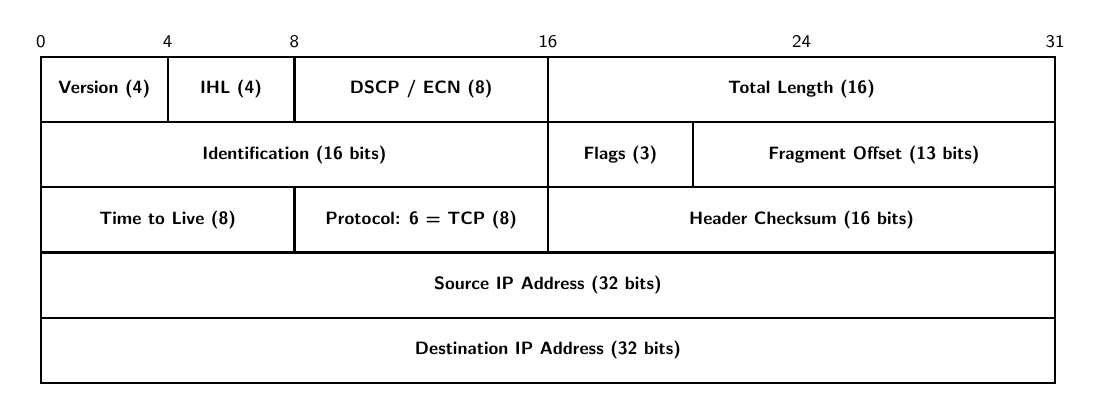
\begin{tikzpicture}[scale=0.92, every node/.style={transform shape}, font=\sffamily\scriptsize]
    \draw[thick] (0, 4.5) rectangle (14, 0);
    \node[above] at (0, 4.5) {0}; \node[above] at (1.75, 4.5) {4}; \node[above] at (3.5, 4.5) {8};
    \node[above] at (7.0, 4.5) {16}; \node[above] at (10.5, 4.5) {24}; \node[above] at (14, 4.5) {31};

    \draw[thick] (0, 3.6) -- (14, 3.6);
    \draw[thick] (1.75, 4.5) -- (1.75, 3.6); \draw[thick] (3.5, 4.5) -- (3.5, 3.6); \draw[thick] (7.0, 4.5) -- (7.0, 3.6);
    \node at (0.875, 4.05) {\textbf{Version (4)}}; \node at (2.625, 4.05) {\textbf{IHL (4)}};
    \node at (5.25, 4.05) {\textbf{DSCP / ECN (8)}}; \node at (10.5, 4.05) {\textbf{Total Length (16)}};

    \draw[thick] (0, 2.7) -- (14, 2.7);
    \draw[thick] (7.0, 3.6) -- (7.0, 2.7); \draw[thick] (9.0, 3.6) -- (9.0, 2.7);
    \node at (3.5, 3.15) {\textbf{Identification (16 bits)}};
    \node at (8.0, 3.15) {\textbf{Flags (3)}}; \node at (11.5, 3.15) {\textbf{Fragment Offset (13 bits)}};

    \draw[thick] (0, 1.8) -- (14, 1.8);
    \draw[thick] (3.5, 2.7) -- (3.5, 1.8); \draw[thick] (7.0, 2.7) -- (7.0, 1.8);
    \node at (1.75, 2.25) {\textbf{Time to Live (8)}};
    \node at (5.25, 2.25) {\textbf{Protocol: 6 = TCP (8)}};
    \node at (10.5, 2.25) {\textbf{Header Checksum (16 bits)}};

    \draw[thick] (0, 0.9) -- (14, 0.9);
    \node at (7.0, 1.35) {\textbf{Source IP Address (32 bits)}};
    \node at (7.0, 0.45) {\textbf{Destination IP Address (32 bits)}};
\end{tikzpicture}
\caption{Layer 3 IPv4 Packet Header Bit Layout (RFC 791, 20 Octets Base).}
\label{fig:header_ipv4}
\end{figure}

\subsubsection{Layer 4: TCP Header \& Active Diagnostic Option Offering}
The TCP segment header conforms to RFC~793. For a bare SYN frame, the base header is 20 octets
($\text{Data Offset} = 5$). However, sending bare SYN probes causes modern operating systems to
suppress advanced protocol capabilities in their SYN/ACK replies. To provoke maximum diagnostic
telemetry for OS fingerprinting, our probe engine formulates a 40-octet frame containing 20
octets of active option offerings (\texttt{STANDARD\_SYN\_OPTIONS}):
\begin{equation}
\text{Options}_{\text{SYN}} = \langle \text{MSS}(1460), \ \text{SACK\_Permitted}, \ \text{Timestamp}(t_0, 0), \ \text{NOP}, \ \text{WScale}(8) \rangle
\end{equation}
Offering these capabilities prompts target operating systems to reveal their compile-time option
ordering, native window scale factors, and timestamp clock frequencies in the return frame.

\begin{figure}[htbp]
\centering
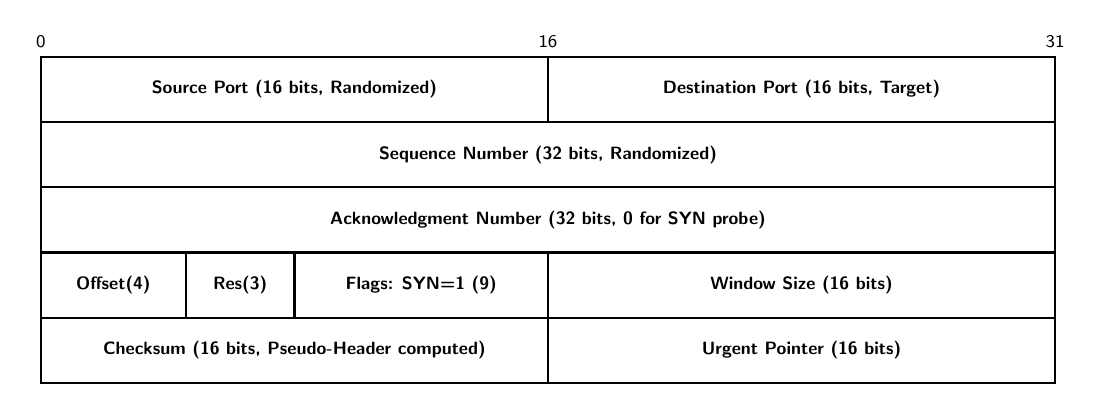
\begin{tikzpicture}[scale=0.92, every node/.style={transform shape}, font=\sffamily\scriptsize]
    \draw[thick] (0, 4.5) rectangle (14, 0);
    \node[above] at (0, 4.5) {0}; \node[above] at (7.0, 4.5) {16}; \node[above] at (14, 4.5) {31};

    \draw[thick] (0, 3.6) -- (14, 3.6); \draw[thick] (7.0, 4.5) -- (7.0, 3.6);
    \node at (3.5, 4.05) {\textbf{Source Port (16 bits, Randomized)}};
    \node at (10.5, 4.05) {\textbf{Destination Port (16 bits, Target)}};

    \draw[thick] (0, 2.7) -- (14, 2.7);
    \node at (7.0, 3.15) {\textbf{Sequence Number (32 bits, Randomized)}};

    \draw[thick] (0, 1.8) -- (14, 1.8);
    \node at (7.0, 2.25) {\textbf{Acknowledgment Number (32 bits, 0 for SYN probe)}};

    \draw[thick] (0, 0.9) -- (14, 0.9);
    \draw[thick] (2.0, 1.8) -- (2.0, 0.9); \draw[thick] (3.5, 1.8) -- (3.5, 0.9); \draw[thick] (7.0, 1.8) -- (7.0, 0.9);
    \node at (1.0, 1.35) {\textbf{Offset(4)}}; \node at (2.75, 1.35) {\textbf{Res(3)}};
    \node at (5.25, 1.35) {\textbf{Flags: SYN=1 (9)}}; \node at (10.5, 1.35) {\textbf{Window Size (16 bits)}};

    \draw[thick] (7.0, 0.9) -- (7.0, 0);
    \node at (3.5, 0.45) {\textbf{Checksum (16 bits, Pseudo-Header computed)}};
    \node at (10.5, 0.45) {\textbf{Urgent Pointer (16 bits)}};
\end{tikzpicture}
\caption{Layer 4 TCP Segment Header Bit Layout (RFC 793, 20 Octets Base).}
\label{fig:header_tcp}
\end{figure}

\subsection{RFC 1071 Checksum Computation \& Pseudo-Header Layout}
Both IPv4 header checksums and TCP segment checksums are computed using our self-authored 16-bit
one's complement algorithm. For TCP, RFC~793 requires prepending a 12-byte IPv4 pseudo-header
to ensure that packets delivered to the wrong host or protocol handler are discarded:
\begin{equation}
\text{Checksum} = \sim \left( \sum_{i=1}^{N} W_i \pmod{2^{16} - 1} \right)
\end{equation}
where $W_i$ denotes consecutive 16-bit binary words across the concatenated pseudo-header and TCP
segment. If the payload length is odd, a null padding octet is appended before summation.

\begin{table}[htbp]
\centering
\small
\renewcommand{\arraystretch}{1.2}
\caption{IPv4 TCP Pseudo-Header Field Layout for Checksum Computation}
\label{tab:pseudo_header}
\begin{tabularx}{\textwidth}{@{}L{2.8cm} L{4.6cm} X@{}}
\toprule
\hdrrow \thh{Byte Offset} & \thh{Field Designation} & \thh{Value Packed in Probe Frame}\\
\midrule
0--3   & Source IPv4 Address      & Bound local interface IP (e.g., \texttt{192.168.0.105})\\
4--7   & Destination IPv4 Address & Target host IP (e.g., \texttt{192.168.0.116})\\
8      & Reserved Octet           & \texttt{0x00}\\
9      & Protocol Identifier      & \texttt{0x06} (\texttt{IPPROTO\_TCP})\\
10--11 & TCP Segment Length       & Total octets of TCP header + options (e.g., 40 octets)\\
\bottomrule
\end{tabularx}
\end{table}

\subsection{Link-Layer Hardware Address Resolution Architecture}
Because standard Windows networking APIs do not expose raw Layer-2 interface bindings directly to
high-level scripts, our toolkit interfaces directly with the native Windows IP Helper library
(\texttt{iphlpapi.dll}) via Python's \texttt{ctypes}:
\begin{enumerate}
    \item \textbf{Local Interface Discovery:} The scanner identifies the active outbound interface
    by creating a connected UDP test socket toward the target subnet and reading \texttt{getsockname()}.
    It then invokes \texttt{GetAdaptersInfo()} to extract the active adapter name, Npcap device GUID,
    and 6-octet hardware MAC address.
    \item \textbf{Pre-Flight Target ARP Resolution:} Prior to probe transmission, the engine
    executes the Windows \texttt{SendARP()} API (passing target IP and MAC output buffer). This
    populates the local ARP cache and retrieves the destination hardware address across the Layer-2
    broadcast domain.
\end{enumerate}
This architecture eliminates the need for hardcoded MAC addresses and allows the raw Ethernet
builder to operate transparently across heterogeneous physical or virtualized interfaces.

\subsection{Operational Safety Rails}\label{sec:safety}
To ensure the toolkit remains strictly an educational reconnaissance instrument and cannot be
misused as an aggressive denial-of-service tool, five non-bypassable safeguards are enforced:
\begin{itemize}
    \item \textbf{RFC~1918 Scope Validation:} Targets are verified via Python's \texttt{ipaddress}
    library; public or routable Internet addresses are rejected immediately.
    \item \textbf{Bounded Probing Horizon:} Probe volume is capped at $\text{MAX\_PROBES} = 50$
    ports per execution run, preventing subnet sweeps or port flooding.
    \item \textbf{Mandatory Rate Limiting:} An inter-probe transmission delay $\ge 0.2$\,s (default
    0.5\,s) is enforced between consecutive packet dispatches.
    \item \textbf{Ephemeral Randomization:} Outbound source ports and initial sequence numbers are
    randomized per probe to prevent state overlap or collision.
    \item \textbf{Reversible Countermeasures:} All active firewall blocks inject bounded TTLs and
    are automatically flushed upon process termination.
\end{itemize}
